% This file was created by matlab2tikz.
%
%The latest updates can be retrieved from
%  http://www.mathworks.com/matlabcentral/fileexchange/22022-matlab2tikz-matlab2tikz
%where you can also make suggestions and rate matlab2tikz.
%
% \documentclass[tikz]{standalone}
% \usepackage[T1]{fontenc}
% \usepackage[utf8]{inputenc}
% \usepackage{pgfplots}
% \usepackage{grffile}
% \pgfplotsset{compat=newest}
% \usetikzlibrary{plotmarks}
% \usepgfplotslibrary{patchplots}
% \usepackage{amsmath}

% \begin{document}
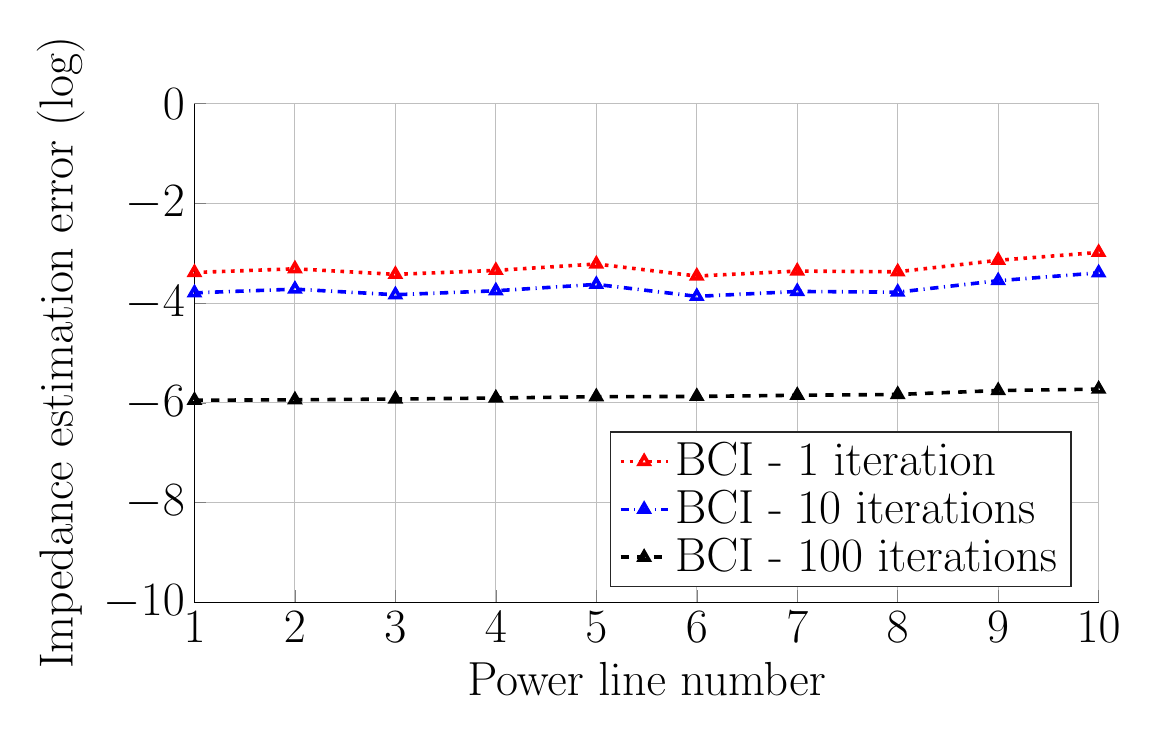
\begin{tikzpicture}

\begin{axis}[%
width=4.521in,
height=2.493in,
% at={(0.758in,0.426in)},
at={(0.758in,0.434in)},
scale only axis,
xmin=1,
xmax=10,
xlabel={Power line number},
xmajorgrids,
ymin=-10,
ymax=0,
% ylabel={$\log_{10}\frac{\|z_n - \hat{z}_n\|_2}{\|z_n\|_2}$},
ylabel={Impedance estimation error (log)},
ymajorgrids,
axis background/.style={fill=white},
axis x line*=bottom,
axis y line*=left,
% legend style={at={(0.5,1.03)},anchor=south,legend cell align=left,align=left,draw=white!15!black},
legend style={legend cell align=left, legend pos=south east, align=right,draw=white!15!black},
xlabel style={font=\LARGE},ylabel style={font=\LARGE},legend style={font=\LARGE},ticklabel style={font=\LARGE}
]

\addplot [color=red,dotted,line width=1.3pt,mark=triangle,mark options={solid}]
  table[row sep=crcr]{%
1	-3.38652769511604\\
2	-3.3125017754448\\
3	-3.42454108436879\\
4	-3.34459142874997\\
5	-3.21636110316632\\
6	-3.45741188077818\\
7	-3.35822040183589\\
8	-3.37239749939876\\
9	-3.14154963894484\\
10	-2.98392482454151\\
};
\addlegendentry{BCI - 1 iteration};

\addplot [color=blue,dashdotted,line width=1.3pt,mark=triangle,mark options={solid}]
  table[row sep=crcr]{%
1	-3.79460707876873\\
2	-3.72099482480146\\
3	-3.83273674153348\\
4	-3.7531238584518\\
5	-3.62532359196459\\
6	-3.86566185875066\\
7	-3.76694141604543\\
8	-3.78111340125635\\
9	-3.55086554012878\\
10	-3.39352482393243\\
};
\addlegendentry{BCI - 10 iterations};

\addplot [color=black,dashed,line width=1.3pt,mark=triangle,mark options={solid}]
  table[row sep=crcr]{%
1	-5.94810422550278\\
2	-5.9401901905404\\
3	-5.92476973786823\\
4	-5.90395647396985\\
5	-5.87782690940461\\
6	-5.8722849057396\\
7	-5.84927456959633\\
8	-5.8329346642505\\
9	-5.7542133357923\\
10	-5.72594239175156\\
};
\addlegendentry{BCI - 100 iterations};

\end{axis}
\end{tikzpicture}%
% \end{document}